% SPDX-License-Identifier: LPPL-1.3c
% Copyright (C) 2026 Christophe Jorssen
% Author and Current Maintainer: Christophe Jorssen <christophe.jorssen@gmail.com>
% LPPL maintenance status: maintained
% This file is part of luafemm. See LICENSE and LICENSES.md for its terms.
\section{Electrostatic sources, views and profiles}
\label{sec:electrostatic}

With its default |model=point charges|, the electric interface evaluates prescribed point charges in a homogeneous,
linear, isotropic medium. All charges lie in the physical $xy$ plane. Its
potential reference is $V(\infty)=0$ and its formulas are
\[
 V(\mathbf r)=\sum_i\frac{q_i}{4\pi\epsilon|\mathbf r-\mathbf r_i|},\qquad
 \mathbf E(\mathbf r)=\sum_i\frac{q_i(\mathbf r-\mathbf r_i)}
 {4\pi\epsilon|\mathbf r-\mathbf r_i|^3},\qquad
 \mathbf D=\epsilon\mathbf E.
\]
Distances in these equations are in metres; public coordinates are converted
using |length unit|. The displayed plane is invariant because the normal field
component vanishes there. The drawn curves are therefore actual field lines
in that plane, not projections of arbitrary three-dimensional curves.

Classical charged spheres, infinite cylinders and ideal capacitors use the
same views and profiles; see Section~\ref{sec:electric-classics}.
For finite electrodes, induced charge and dielectric interfaces, select
|model=finite elements| as described in Section~\ref{sec:electric-fe}.

There is no finite-element mesh, induced conductor charge, dielectric interface,
periodic boundary, or external circuit in this model. Magnetic |femm/region|,
|femm/boundary| and |femmsolve| commands do not configure an electric model.
Use separate electric and magnetic pictures. FEMM's native planar point-source
conventions do not describe these three-dimensional charges; this interface
provides neither native FEM/ANS nor FEE/RES export.

\subsection{Models and ownership}
\label{sec:electric-model}
\begin{key}{/tikz/femm/electrostatic=\marg{options} (default \{\})}
Set on a |tikzpicture| before its begin hook. The options belong to
|/femm/electrostatic|. The key sets TikZ's drawing basis to |x=1cm,y=1cm|;
put your own |x| and |y| options after it to override the display basis.
Unequal display axes can distort angles and circles on paper without changing
the physical model. The root transform is a view transform; local transforms inside the picture
move physical sources relative to that root. Repeated configuration keys in the
picture options merge before one model is created.
\end{key}

Declare sources first. The first field, vector, contour or profile request
freezes the list. Later source declarations fail. Seed contours and ordinary
annotations do not add physical sources. Names and profiles have document
lifetime, whereas PGF key settings retain ordinary TeX grouping. Reusing a
snapshot or profile name replaces that name atomically; previous profiles own
their data and do not change. There is no disk cache or persistent electric
snapshot file in this interface.

\begin{key}{/femm/electrostatic/length unit=\meta{unit} (initially cm)}
Choice |m|, |cm|, |mm| or |um|. One model coordinate equals this physical
length. This choice is independent of the size of the figure on paper.
Set before the picture begins.
\end{key}

\begin{key}{/femm/electrostatic/relative permittivity=\meta{number} (initially 1)}
Positive dimensionless $\epsilon_r$, with
$\epsilon=\epsilon_0\epsilon_r$ and
$\epsilon_0=8.8541878128\times10^{-12}\,\mathrm{F/m}$.
The default represents vacuum. No electric material is inferred from the
magnetic material catalogue.
\end{key}

\begin{key}{/femm/electrostatic/xmin=\meta{coordinate} (initially -3)}
Default view-window edge in model units. The minima must be strictly smaller
than the maxima. For analytical models this is a crop: charges outside it still contribute.
For |model=finite elements| these four keys instead define the physical
computational rectangle; crop the view with |/femm/electric/xmin| and its peers.
\end{key}

\begin{key}{/femm/electrostatic/xmax=\meta{coordinate} (initially 3)}
Default view-window edge in model units. The minima must be strictly smaller
than the maxima. For analytical models this is a crop: charges outside it still contribute.
For |model=finite elements| these four keys instead define the physical
computational rectangle; crop the view with |/femm/electric/xmin| and its peers.
\end{key}

\begin{key}{/femm/electrostatic/ymin=\meta{coordinate} (initially -2)}
Default view-window edge in model units. The minima must be strictly smaller
than the maxima. For analytical models this is a crop: charges outside it still contribute.
For |model=finite elements| these four keys instead define the physical
computational rectangle; crop the view with |/femm/electric/xmin| and its peers.
\end{key}

\begin{key}{/femm/electrostatic/ymax=\meta{coordinate} (initially 2)}
Default view-window edge in model units. The minima must be strictly smaller
than the maxima. For analytical models this is a crop: charges outside it still contribute.
For |model=finite elements| these four keys instead define the physical
computational rectangle; crop the view with |/femm/electric/xmin| and its peers.
\end{key}

\begin{key}{/femm/electrostatic/name=\meta{name} (initially \normalfont empty)}
Save an owned electric snapshot at the end of the picture. A snapshot
contains charges and exclusion radii (or classical geometry and source data),
physical metadata and its original view
window. FE snapshots additionally own the mesh, solution and physical paths. The name may contain spaces. Omitting it creates no named snapshot.
\end{key}

\begin{key}{/femm/electrostatic/snapshot=\meta{name} (initially \normalfont empty)}
Start from a previously named frozen snapshot, with the new picture's
transform and requested window. Do not declare additional charge nodes.
The |length unit| and |relative permittivity| options must match the snapshot;
repeat their nondefault values explicitly. Mismatches are errors.
\end{key}

\begin{codeexample}[width=0pt]
\begin{tikzpicture}[femm/electrostatic={length unit=mm,
    relative permittivity=3,name=small charge,
    xmin=-4,xmax=4,ymin=-2,ymax=2},x=5mm,y=5mm]
  \node[femm/point charge={charge=1e-12,exclusion radius=.5},
    minimum size=3mm] at (0,0) {$+$};
  \pic[femm/electric={lines per charge=8}] {femm electric field};
\end{tikzpicture}
\begin{tikzpicture}[femm/electrostatic={snapshot=small charge,
    length unit=mm,relative permittivity=3,
    xmin=-4,xmax=4,ymin=-2,ymax=2},x=5mm,y=5mm]
  \pic[femm/electric={levels={1,2,3},contour resolution=60}]
    {femm equipotentials};
\end{tikzpicture}
\end{codeexample}

\subsection{The point-charge node}
\label{sec:electric-charge}
\begin{key}{/tikz/femm/point charge=\marg{options}}
Apply style |femm charge| and the PGF shape |femm point charge| to an ordinary
node, and parse |/femm/point charge| options. An electric picture is required.
Registration happens once, in the final shape drawing frame. Standard circle
anchors, including |center|, compass anchors, |text|, |base| and |mid|, remain
available; consulting them does not create charges. A noncentral |anchor|
changes the source position because the source remains at the actual centre.
Matrix/delayed node placement is rejected: its final physical position is not
available at the capture hook. Ordinary immediately placed nodes and loops are
supported.
\end{key}

\begin{key}{/femm/point charge/charge=\meta{PGF expression} (initially \normalfont required)}
Signed charge in coulombs. PGF's floating-point parser evaluates expressions,
including scientific notation such as |charge=-2e-9|. There is no implicit
charge inferred from the text or colour of the node. Zero charge contributes
nothing; exactly coincident charges are summed, and a zero sum removes the
singularity. Distinct centres are never merged merely because they are close.
\end{key}

\begin{key}{/femm/point charge/exclusion radius=\meta{PGF expression} (initially .22)}
Positive radius in model coordinate units. Field lines stop outside this
source mask; vectors and profiles omit it, and contour cells touching it are
removed. This masks the singularity without softening Coulomb's law. The
physical source remains a point. Changing |minimum size|, |inner sep| or
|transform shape| does not change this radius or the charge.
\end{key}

\begin{key}{/tikz/femm charge=\meta{style}}
Ordinary composable TikZ style: a white symbol with a grey outline, minimum
size 4\,mm, inner separation 1\,pt and outer separation .5\,pt. Use
|femm charge/.append style| for defaults and ordinary node options for local
changes. The underlying shape can also be selected as |shape=femm point charge|
when the charge family is configured separately.
\end{key}

\begin{codeexample}[width=0pt]
\begin{tikzpicture}[femm/electrostatic={},rotate=20,
    femm charge/.append style={fill=red!15,minimum size=5mm}]
  \begin{scope}[shift={(.5,0)}]
    \node[femm/point charge={charge=2*1e-9},anchor=west] (q) at (0,0) {$+$};
  \end{scope}
  \draw[gray,->] (-1,1)--(q.north);
  \draw[gray] (q.center) circle[radius=.22];
  \path[femm/electric seeds={samples=5}] (-2,-1)--(-2,1);
  \pic {femm electric field};
\end{tikzpicture}
\end{codeexample}

\subsection{Electric views}
\label{sec:electric-view}
\begin{key}{/tikz/femm/electric=\marg{options}}
Configure the scoped family |/femm/electric|. Put it on a picture, scope or
individual pic. Source coordinates always belong to the enclosing electric
model: a pic's own |at|, rotation or scaling does not reposition physical data.
Configure the picture transform to move a whole view.
\end{key}

\begin{key}{/tikz/pics/femm electric field}
Integrate oriented field lines. Invoke as |\pic {femm electric field};| after all source nodes.
\end{key}

\begin{key}{/tikz/pics/femm equipotentials}
Extract contours of electric scalar potential. Invoke as |\pic {femm equipotentials};| after all source nodes.
\end{key}

\begin{key}{/tikz/pics/femm electric vectors}
Draw arrows sampling the electric field. Invoke as |\pic {femm electric vectors};| after all source nodes.
\end{key}

\begin{key}{/tikz/femm electric field=\meta{style}}
Drawing style, initially blue, .4\,pt, with the electric orientation arrow decoration. Use |/.style| or |/.append style| to customise it.
Shared |femm/arrows|, |femm/arrow spacing|, |femm/arrow length| and
|femm/arrow width| also configure electric field-line arrows.
\end{key}

\begin{key}{/tikz/femm equipotential=\meta{style}}
Drawing style, initially orange, densely dashed, .35\,pt. Use |/.style| or |/.append style| to customise it.
Shared |femm/arrows|, |femm/arrow spacing|, |femm/arrow length| and
|femm/arrow width| also configure electric field-line arrows.
\end{key}

\begin{key}{/tikz/femm electric vector=\meta{style}}
Drawing style, initially blue-green, .4\,pt, with a Stealth tip. Use |/.style| or |/.append style| to customise it.
Shared |femm/arrows|, |femm/arrow spacing|, |femm/arrow length| and
|femm/arrow width| also configure electric field-line arrows.
\end{key}

\begin{key}{/femm/electric/xmin=\meta{coordinate} (initially \normalfont empty)}
Optional view edge in model units, overriding the enclosing model's default
window for this pic. An empty value inherits that edge. This never excludes
charges from the calculation.
\end{key}

\begin{key}{/femm/electric/xmax=\meta{coordinate} (initially \normalfont empty)}
Optional view edge in model units, overriding the enclosing model's default
window for this pic. An empty value inherits that edge. This never excludes
charges from the calculation.
\end{key}

\begin{key}{/femm/electric/ymin=\meta{coordinate} (initially \normalfont empty)}
Optional view edge in model units, overriding the enclosing model's default
window for this pic. An empty value inherits that edge. This never excludes
charges from the calculation.
\end{key}

\begin{key}{/femm/electric/ymax=\meta{coordinate} (initially \normalfont empty)}
Optional view edge in model units, overriding the enclosing model's default
window for this pic. An empty value inherits that edge. This never excludes
charges from the calculation.
\end{key}

\begin{key}{/femm/electric/lines per charge=\meta{integer} (initially 16)}
Number of equally spaced angular seeds per selected charge, from 1 to 1000.
Seeds lie at 1.05 times the source exclusion radius. This is aesthetic seeding,
not flux weighting. Explicit seeds replace this automatic set.
\end{key}

\begin{key}{/femm/electric/seed sign=\meta{choice} (initially auto)}
Choose |auto|, |positive|, |negative| or |all|. Automatic seeding uses positive
charges if any exist, otherwise negative charges. With |all| a connecting line
may be drawn twice, from independently selected endpoints. Seeding only one sign
does not generally find every line entering from or leaving towards infinity.
\end{key}

\begin{key}{/femm/electric/seeds=\marg{x/y,\ldots} (initially \normalfont empty)}
Explicit model-coordinate seeds, for example |seeds={0/1,0/-1}|.
They override a previously captured seed contour, which in turn overrides
automatic charge seeds. Sources outside the plotting window still contribute;
seeds outside it produce no line.
\end{key}

\begin{key}{/femm/electric/direction=\meta{choice} (initially both)}
Integrate |forward|, |backward| or |both| from each seed. Backward integration
follows $-\mathbf E$ to find the earlier part of a line, but the final polyline
is reversed so that all arrows still point along $\mathbf E$.
\end{key}

\begin{key}{/tikz/femm electric oriented field}
Arrow-decoration style used by |femm electric field|. It observes |femm/arrows|
and the shared arrow dimensions and spacing. Its initial mark is further from
source symbols than the magnetic contour decoration.
\end{key}

\begin{key}{/femm/electric/arrow position=\meta{fraction} (initially .45)}
First arrow at this fraction of total line length, between 0 and .95.
Further arrows use |femm/arrow spacing| up to fraction .95. Raise the fraction
to keep short source-to-boundary lines clear of their charge symbol.
\end{key}

\begin{key}{/femm/electric/step=\meta{number} (initially .08)}
Maximum integration step in model units. Other steps adapt automatically. These controls do not change the analytical field.
\end{key}

\begin{key}{/femm/electric/tolerance=\meta{number} (initially .0001)}
Positive absolute local position-error tolerance in model units. It also controls near-source termination. Other steps adapt automatically. These controls do not change the analytical field.
\end{key}

\begin{key}{/femm/electric/max length=\meta{number} (initially 40)}
Positive maximum arclength in model units, separately for each direction from a seed. Other steps adapt automatically. These controls do not change the analytical field.
\end{key}

\begin{key}{/femm/electric/max steps=\meta{number} (initially 10000)}
Accepted-step budget per integration direction, an integer from 1 to 1000000. Exhaustion emits a log warning and returns the truncated line. Other steps adapt automatically. These controls do not change the analytical field.
\end{key}

\begin{key}{/femm/electric/null field=\meta{number} (initially 1e-9)}
Positive field threshold in V/m below which direction is undefined for tracing and arrows. Other steps adapt automatically. These controls do not change the analytical field.
\end{key}

\begin{key}{/femm/electric/contour resolution=\meta{integer} (initially 80)}
Number of grid cells horizontally, from 4 to 1000. The vertical count follows
the window aspect ratio, with at least four cells. The total grid is limited to
one million sample points. Each rectangle is split into two triangles; scalar
intersections are connected across shared edges. Raise the resolution to reduce
polygonal contour error and to recover features smaller than a cell.
\end{key}

\begin{key}{/femm/electric/levels=\marg{voltages} (initially \normalfont empty)}
Comma-separated finite potential levels in volts, up to 100 distinct values.
An empty list uses automatic levels. Specify levels when comparing figures;
automatic levels depend on the view window, resolution and exclusion masks.
\end{key}

\begin{key}{/femm/electric/level count=\meta{integer} (initially 11)}
Automatic level count from 1 to 100. Levels lie strictly inside the sampled
unmasked range. If that range includes both signs, the smaller absolute extreme
sets symmetric bounds. A constant potential gives no automatic contours.
Explicit |levels| takes precedence.
\end{key}

\begin{key}{/femm/electric/vector spacing=\meta{number} (initially .5)}
Positive square-grid spacing in model units. Samples are offset half a spacing
from the lower window edges. The sampling budget is 100000 arrows.
\end{key}

\begin{key}{/femm/electric/vector mode=\meta{choice} (initially normalized)}
Choose |normalized| for equal-length direction arrows, or |scaled| for lengths
proportional to $|\mathbf E|$. Arrows that would cross a source mask or leave
the window are omitted rather than shortened to a false quantitative length.
\end{key}

\begin{key}{/femm/electric/vector length=\meta{number} (initially .28)}
Positive arrow length in model units for |vector mode=normalized|.
It is ignored in scaled mode.
\end{key}

\begin{key}{/femm/electric/vector scale=\meta{number} (initially 1e-5)}
Positive model-coordinate length per V/m for |vector mode=scaled|.
Supply a reference arrow or state the scale for quantitative interpretation.
It is ignored in normalized mode.
\end{key}

\begin{codeexample}[width=0pt]
\begin{tikzpicture}[femm/electrostatic={xmin=-2,xmax=2},
    femm equipotential/.append style={gray},
    femm electric vector/.append style={black},
    femm electric field/.append style={violet},
    femm/arrow spacing=12mm]
  \node[femm/point charge={charge=-1e-9},fill=blue!15] at (0,0) {$-$};
  \pic[femm/electric={xmin=-1.8,xmax=1.8,ymin=-1.6,ymax=1.6,
    vector mode=scaled,vector scale=.00002,vector spacing=.6}]
    {femm electric vectors};
  \pic[femm/electric={level count=4,contour resolution=60}]
    {femm equipotentials};
  \pic[femm/electric={seeds={-1/1,1/1},direction=backward,
    max length=2,max steps=3000,null field=1e-8,step=.04,tolerance=.00001}]
    {femm electric field};
\end{tikzpicture}
\end{codeexample}

\subsection{Contours, profiles and PGFPlots}
\label{sec:electric-profile}
\begin{key}{/tikz/femm/electric profile=\marg{options}}
Capture one connected TikZ path as an electric profile.
Its options belong to the |/femm/electric profile| family. Open paths, arcs, closed paths and cubic curves are
supported. Capture uses the evaluated soft path after transformations and
rounded corners. Samples are equally spaced in the flattened path's arclength.
The physical model freezes at capture; values and source data are owned by the
profile, independently of subsequent pictures.
\end{key}

\begin{key}{/tikz/femm/electric seeds=\marg{options}}
Capture one path as seed positions for subsequent field pics in this picture.
Uses the same option family as profiles, with |samples=16| unless overridden.
Only |samples| and |curve tolerance| apply; it creates no named profile and does
not freeze charges. A later seed contour replaces the earlier one. Closed paths
repeat their endpoint; omit an endpoint or use an open arc to avoid a duplicate
seed when this matters.
\end{key}

\begin{key}{/femm/electric profile/name=\meta{name} (initially \normalfont required for profiles)}
Document-wide profile name. Reusing the name replaces the profile, while
already emitted plots are unchanged. Ignored for seed-contour capture.
\end{key}

\begin{key}{/femm/electric profile/samples=\meta{integer} (initially 201)}
Uniform arclength sample count, including both endpoints, from 2 to 100000.
Seed capture initially uses 16 instead. Under |outside=nan|, extra gap samples
are inserted if necessary so a narrow excluded disk cannot be crossed by a
spurious plotted segment between two ordinary samples.
\end{key}

\begin{key}{/femm/electric profile/curve tolerance=\meta{number} (initially .001)}
Positive geometric flattening tolerance in model units. This controls the
measurement or seed path, independently of field-line integration tolerance
and equipotential resolution.
\end{key}

\begin{key}{/femm/electric profile/outside=\meta{choice} (initially error)}
Choose |error| to reject a profile touching a source exclusion disk or an
invalid analytical value, or |nan| to create explicit gaps. Analytical profiles
may extend beyond the view window. The policy concerns invalid field locations,
not picture cropping. Ignored for geometrical seed capture.
\end{key}

\begin{command}{\femmelectricplot\opt{\oarg{options}}}
Inside an ordinary PGFPlots axis, emit an |\addplot+| from a named electric
profile. Options use |/femm/electric plot| and obey TeX scope. Cycle lists,
legends, axis units, formatting and transformations remain ordinary PGFPlots
features. |unbounded coords=jump| preserves gaps by default; do not override it
with a policy that joins across singularities.
\end{command}
\begin{key}{/femm/electric plot/profile=\meta{name} (initially \normalfont required)}
Previously captured electric profile. A later magnetic or electric picture
does not change its source data.
\end{key}

\begin{key}{/femm/electric plot/component=\meta{choice} (initially E)}
Choose |V| (volts), |E|, |Ex| or |Ey| (V/m), or |D|, |Dx| or |Dy|
(C/m$^2$). |E| and |D| are nonnegative magnitudes. Cartesian components refer
to the model's physical frame, not a rotated display frame. The normal-to-plane
component is identically zero for this coplanar provider.
\end{key}

\begin{key}{/femm/electric plot/abscissa=\meta{choice} (initially s)}
Choose arclength |s| from the contour start, Cartesian |x| or |y|, all in
model coordinate units, or normalized arclength |t| from zero to one.
There is no implicit conversion to metres on the plotting axis.
\end{key}

\begin{key}{/femm/electric plot/plot options=\marg{PGFPlots options} (initially \normalfont empty)}
Ordinary |\addplot+| options, passed without numerical interpretation.
Use these for colour, thickness, mark style and other PGFPlots controls.
\end{key}

\begin{codeexample}[width=0pt]
\begin{tikzpicture}[femm/electrostatic={}]
  \node[femm/point charge={charge=1e-9}] at (0,0) {$+$};
  \draw[densely dotted,femm/electric profile={name=through charge,
    samples=100,outside=nan,curve tolerance=.0005}] (-2,0)--(2,0);
\end{tikzpicture}
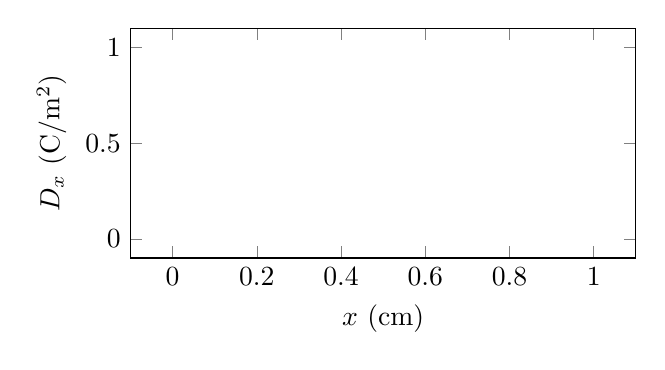
\begin{tikzpicture}
  \begin{axis}[width=8cm,height=4.5cm,no markers,
    xlabel={$x$ (cm)},ylabel={$D_x$ (C/m$^2$)}]
    \femmelectricplot[profile=through charge,component=Dx,abscissa=x,
      plot options={green!45!blue,thick}]
  \end{axis}
\end{tikzpicture}
\end{codeexample}

\subsection{Numerical conventions and Lua contracts}
\label{sec:electric-method}
Coulomb evaluation is direct superposition, with no mesh and no softened source.
An evaluation at a nonzero source returns an invalid-point diagnostic.
Very large inputs producing overflow also fail to produce a field value.
Exactly cancelled coincident sources are removed before evaluation.

Field curves use adaptive fourth-order Runge--Kutta integration of
$\mathrm d\mathbf r/\mathrm ds=\mathbf E/|\mathbf E|$, comparing one full step
with two half steps. They stop at the view boundary, near a source mask, at an
unresolved critical point, at the specified field threshold, or at the length
or step budget. No direction is invented at a null point. An almost critical
line may require a smaller step or tolerance to resolve its separation from a
separatrix. Field-line density in this plane is not a measure of 3D flux.

Equipotentials interpolate sampled scalar values on a triangular grid.
Cells intersecting an exclusion disk are conservatively omitted; this can make
a visible gap larger than the disk by roughly a cell. Refine the grid to reduce
that effect. A coarse grid can miss small level loops and closely spaced
features. Profiles instead evaluate the analytical kernel along their
flattened path, independently of contour resolution. Check curve flattening
and sample spacing when a path or field varies rapidly.

The format-neutral module |luafemm-physical| supplies |describe| and |sample|.
Its magnetic sampling adapter is limited to solved real planar/axisymmetric FE
fields; phasor, axial and ideal-circuit views retain their existing dedicated APIs.
Descriptors distinguish physics, provider, three-dimensional physical law,
two-dimensional evaluation, length scale, SI observable units, potential
reference, homogeneous medium and validity set. Electric builders and owned
snapshots live in |luafemm-electrostatic|; rendering geometry lives separately
in |luafemm-electric-view|. The TeX adapter owns name registries and serializes
numeric geometry into PGF paths. It never executes user-provided Lua expressions.
This descriptor contract is not an on-disk file format.

For Lua use, |new| takes |length_unit| and |epsilon_r| plus view bounds.
Call |add| with model, coordinates, charge and radius to add a source.
Then |freeze| closes the builder;
|snapshot| returns an independent frozen copy. |sample(model,x,y)| returns
|V|, |Ex|, |Ey|, |E|, |Dx|, |Dy| and |D| in SI, or |nil,reason| at an invalid
point. Raw |sample| ignores drawing masks and the plotting window; it freezes
its source list before its first evaluation. Descriptors returned by |describe|
are copies. No native solver, database or external plotting program is needed.
